\PassOptionsToPackage{disable}{microtype}
\documentclass[sigconf,nonacm]{acmart}

\setcopyright{none}
\settopmatter{printacmref=false}
\renewcommand\footnotetextcopyrightpermission[1]{}
\pagestyle{plain}
\hfuzz=20pt

\usepackage{booktabs}
\usepackage{tabularx}
\usepackage{multirow}
\usepackage{amsmath}
\let\Bbbk\relax
\usepackage{amssymb}
\usepackage{algorithm}
\usepackage{algorithmic}
\usepackage{tikz}
\usepackage{pgfplots}
\pgfplotsset{compat=1.18}
\usepackage{url}
\urlstyle{rm}

\usetikzlibrary{arrows.meta,positioning,calc,shapes.geometric,
                decorations.pathreplacing,patterns,fit,backgrounds}

\definecolor{cblu} {RGB}{ 50,110,190}
\definecolor{cgrn} {RGB}{ 40,150, 70}
\definecolor{cora} {RGB}{210,110, 30}
\definecolor{cred} {RGB}{200, 50, 50}
\definecolor{cyel} {RGB}{190,165,  0}
\definecolor{cpur} {RGB}{130, 50,170}
\definecolor{cgry} {RGB}{100,100,100}

\begin{CCSXML}
<ccs2012>
  <concept>
    <concept_id>10002978.10002991.10002993</concept_id>
    <concept_desc>Security and privacy~Cryptanalysis and other attacks</concept_desc>
    <concept_significance>500</concept_significance>
  </concept>
  <concept>
    <concept_id>10002978.10002991.10002995</concept_id>
    <concept_desc>Security and privacy~Public key (asymmetric) techniques</concept_desc>
    <concept_significance>500</concept_significance>
  </concept>
  <concept>
    <concept_id>10010147.10010257.10010293</concept_id>
    <concept_desc>Computing methodologies~Machine learning</concept_desc>
    <concept_significance>300</concept_significance>
  </concept>
  <concept>
    <concept_id>10011007.10011074.10011099</concept_id>
    <concept_desc>Software and its engineering~Software verification and validation</concept_desc>
    <concept_significance>300</concept_significance>
  </concept>
</ccs2012>
\end{CCSXML}

\ccsdesc[500]{Security and privacy~Cryptanalysis and other attacks}
\ccsdesc[500]{Security and privacy~Public key (asymmetric) techniques}
\ccsdesc[300]{Computing methodologies~Machine learning}
\ccsdesc[300]{Software and its engineering~Software verification and validation}

\title{AI-Powered Cryptographic Discovery and Inventory: A Multi-Modal Framework for CBOM Generation in Post-Quantum Migration}

\author{Ezekiel Ologunde}
\affiliation{%
  \institution{Independent Researcher}
  \city{Boston}
  \state{MA}
  \country{USA}}
\email{ologunde@bu.edu}

\begin{abstract}
\sloppy
The transition to post-quantum cryptography (PQC) is no longer a future
problem. NIST has finalised three PQC standards (ML-KEM/FIPS-203,
ML-DSA/FIPS-204, SLH-DSA/FIPS-205) in 2024, and federal procurement
guidance under the National Security Memorandum 10 mandates migration
timelines that begin biting in 2027--2030. The bottleneck blocking
organisational migration, however, is not algorithm availability: it is
\emph{cryptographic visibility}. Organisations cannot replace
quantum-vulnerable algorithms they cannot find, and cryptographic usage
is dispersed across source code, compiled binaries, firmware images, and
encrypted network traffic with no canonical inventory in any production
environment. This paper presents \textsc{CryptoLens}, an AI-driven
framework for automated cryptographic discovery generating a structured
Cryptographic Bill of Materials (CBOM) compliant with the CycloneDX 1.6
specification. \textsc{CryptoLens} integrates four discovery channels:
CodeBERT-based source-code analysis, ML-augmented binary and firmware
analysis with constant-pattern recognition and library fingerprinting,
deep learning on TLS handshake metadata, and a unified inventory
constructor with quantum-vulnerability risk scoring. We evaluate on a
corpus combining 4{,}200 open-source repositories, 1{,}847 firmware
images, and 18 months of network captures from partner enterprises.
\textsc{CryptoLens} achieves 0.918 cryptographic-API recall on source
(versus 0.624 for regex baselines), identifies cryptographic functions
in 87\% of unstripped binaries and 71\% of stripped firmware, classifies
TLS cipher suites with 0.964 accuracy from metadata alone, and produces
deduplicated CBOMs that are 3.2$\times$ more complete than the strongest
commercial baseline. We document operational deployment patterns
including CI/CD integration, drift detection, and the unresolved
ground-truth problem that limits formal completeness claims. The
contribution is positioned for direct alignment with NIST NCCoE,
CISA PQC migration, and CycloneDX standardisation programmes.
\end{abstract}

\keywords{post-quantum cryptography, CBOM, CycloneDX, cryptographic
discovery, binary analysis, firmware analysis, TLS fingerprinting,
PQC migration, ML-KEM, ML-DSA, harvest-now-decrypt-later}

\begin{document}
\maketitle
\sloppy
\tolerance=9999
\emergencystretch=3em
\hfuzz=10pt

\section{Introduction}

The post-quantum cryptography transition has crossed from research topic
to executable mandate. NIST's August 2024 publication of FIPS-203
(ML-KEM, formerly Kyber), FIPS-204 (ML-DSA, formerly Dilithium), and
FIPS-205 (SLH-DSA, formerly SPHINCS+) finalised three standardised
post-quantum algorithms~\cite{nist2024fips203,nist2024fips204,nist2024fips205}.
The accompanying CNSA 2.0 advisory~\cite{nsa2024cnsa2} requires
National Security Systems to begin transition by 2027 and complete it
by 2030--2033 depending on system class. The 2022 National Security
Memorandum 10~\cite{whitehouse2022nsm10} extends similar pressure
across federal civilian systems. Commercial deployments outside the
federal scope face the parallel pressure of \emph{harvest-now,
decrypt-later} attacks: encrypted traffic captured today and stored
against the eventual availability of cryptographically relevant quantum
computers~\cite{mosca2024quantum}.

The defensive response has, however, run into a structural problem
that no amount of algorithm engineering solves: organisations do not
know where their existing cryptography is. Cryptographic usage is
distributed across source code (statically analysable but often
obfuscated through indirection and abstraction layers), compiled
binaries (where direct visibility into algorithm choice is lost
without dedicated analysis), firmware images (where binaries are
typically stripped and may use custom or vendor-specific libraries),
and encrypted network protocols (where the encryption itself
obscures the cryptographic configuration in
use)~\cite{nccoe2024cryptodisc,heron2024visibility}. Production
environments routinely contain thousands of services, hundreds of
thousands of binaries, and millions of source files; manual
cryptographic inventory at this scale is infeasible.

\subsection{The Visibility Bottleneck}

The cryptographic visibility problem manifests in three operational
failure modes that the PQC migration literature has begun to
document:

\textbf{Forgotten dependencies}. RSA-2048 keys generated for
internal services in the 2010s remain in production despite the
service teams that owned them having since reorganised, the
documentation having been lost, and the keys appearing in no
current configuration management
database~\cite{wisser2024forgotten}.

\textbf{Indirect cryptographic usage}. A service may not directly call
RSA functions but uses a TLS library that uses an X.509 library that
uses an RSA library three layers down. The cryptographic dependency
is real; the visibility into it via direct code inspection is poor.

\textbf{Vendor and firmware blind spots}. Network appliances,
embedded systems, and IoT devices often ship with proprietary
cryptographic implementations whose algorithm choices are
documented only in vendor specification sheets that may not be
machine-readable or even available.

The combination of these failure modes is that even an organisation
that wants to migrate to PQC cannot enumerate its current
cryptographic surface in actionable detail. Migration cannot begin
without enumeration; enumeration is the precondition the field has
been treating as a free input.

\subsection{Contributions}

This paper presents \textsc{CryptoLens}, a multi-modal AI-driven
cryptographic discovery framework whose contributions are:

\begin{itemize}
  \item A four-channel discovery architecture covering source code
        (CodeBERT-based), compiled binaries (ML-augmented static
        analysis with constant-pattern detection), firmware images
        (specialised stripped-binary classifier), and encrypted
        network traffic (TLS metadata classifier).
  \item A unified CBOM constructor producing CycloneDX 1.6-compliant
        output with deduplication, dependency mapping, and
        quantum-vulnerability risk scoring aligned to the NIST PQC
        algorithm classification.
  \item Empirical evaluation on 4{,}200 repositories, 1{,}847 firmware
        images, and 18 months of partner enterprise network captures
        demonstrating substantial coverage improvement over
        regex-based and signature-based baselines.
  \item A specific analysis of \emph{indirect} cryptographic usage
        through dependency-resolution that source-code-only and
        binary-only methods systematically miss.
  \item Deployment-pattern guidance covering CI/CD integration,
        continuous drift detection, and the operationally-correct way
        to handle the absent-ground-truth problem.
  \item Explicit alignment with NIST NCCoE Migration to Post-Quantum
        Cryptography project~\cite{nccoe2024cryptodisc}, CISA PQC
        guidance~\cite{cisa2024pqc}, and CycloneDX 1.6
        cryptography asset standardisation~\cite{cyclonedx2024crypto}.
\end{itemize}

\section{Background and Related Work}

\subsection{The CBOM Standard}

The Cryptographic Bill of Materials (CBOM) specification, formalised
within CycloneDX 1.6 in 2024~\cite{cyclonedx2024crypto}, extends the
SBOM concept to cryptographic assets. A CBOM enumerates:

\textbf{Algorithms}: cryptographic primitives in use (RSA, ECDSA,
AES, SHA-2, ML-KEM, etc.) with parameter specifications (key sizes,
elliptic curves, mode of operation).

\textbf{Cryptographic libraries}: implementations providing the
algorithms (OpenSSL, BoringSSL, Bouncy Castle, libsodium) with
version information.

\textbf{Cryptographic assets}: keys, certificates, and other
cryptographic material with contextual metadata (purpose, expiration,
classification level).

\textbf{Usage context}: where each asset is used (authentication,
encryption, signing, key exchange) and which application components
depend on it.

\textbf{Quantum-vulnerability classification}: per-asset assessment of
whether the asset is quantum-vulnerable (RSA, ECC, DH), classical-only
(symmetric, hash) but at-risk (AES-128 reduced to 64-bit security under
Grover), or post-quantum-safe (ML-KEM, ML-DSA, hash-based signatures).

The CycloneDX 1.6 specification provides the schema; production
\emph{generation} of CBOMs from real systems remains an open problem
the present work addresses.

\subsection{Prior Cryptographic Discovery Work}

The discovery literature is fragmented across modality-specific tools:

\textbf{Source-level discovery}: rule-based scanners
(IBM CBOMkit~\cite{ibm2024cbomkit}, Sonatype's Lift) that match
cryptographic API patterns. Effective for canonical patterns; brittle
to indirection, custom wrappers, and abstracted cryptographic
operations.

\textbf{Binary-level discovery}: BinSight~\cite{caballero2023binsight}
and Cryptosense~\cite{cryptosense2024} apply signature matching and
constant-pattern detection. State of the art achieves 60--75\% recall
on stripped binaries.

\textbf{Network-level discovery}: passive TLS inspection tools
(JA3, JARM~\cite{salesforce2024jarm}) classify cipher suite
distributions but do not produce structured inventory output.

\textbf{Recent ML-based work}: Kim et al.~\cite{kim2024deepbin}
applied transformer architectures to binary cryptographic function
identification with 0.86 F1 on stripped x86. Liu et
al.~\cite{liu2025cryptoid} applied CodeBERT fine-tuning to
cryptographic API identification across multiple programming languages.

What is missing across this body of work is a unified multi-modal
framework that integrates all four channels into a coherent CBOM
output with quantum-vulnerability scoring. \textsc{CryptoLens} fills
this gap with an architecture explicitly designed for the operational
PQC migration problem.

\subsection{Policy and Funding Landscape}

The cryptographic discovery problem is recognised at policy level:

\textbf{NIST NCCoE}: the Migration to Post-Quantum Cryptography
project~\cite{nccoe2024cryptodisc} explicitly identifies
``cryptographic discovery and inventory'' as a critical capability
gap and is funding industry-academic collaborations in this area.

\textbf{CISA}: 2024 PQC migration guidance~\cite{cisa2024pqc}
identifies inventory as the first phase of migration; the agency's
2024 CDM (Continuous Diagnostics and Mitigation) extension
budget includes cryptographic asset visibility.

\textbf{NSA CNSA 2.0}: requires National Security Systems to
maintain ``machine-actionable cryptographic
inventories''~\cite{nsa2024cnsa2}, language directly aligned with
CBOM standardisation.

The combination of recognised problem, finalised algorithms, and
mandated migration timelines makes this an unusually well-funded
research environment.

\section{Threat Model and Scope}

\subsection{The Adversary Behind the Mandate}

The motivating adversary is the cryptographically-relevant quantum
computer (CRQC). Estimates of CRQC arrival vary
widely~\cite{mosca2024quantum,gidney2025quantumlogic}; the
operationally relevant property is not the precise arrival date but
that two adversary capabilities exist already:

\textbf{Harvest-now-decrypt-later}. An adversary can capture
encrypted traffic today, store it indefinitely, and decrypt it once
sufficient quantum capability becomes available. Data with long
confidentiality lifetimes (medical records, classified material,
intellectual property) is at risk now even if CRQC is decades
away~\cite{mosca2024quantum}.

\textbf{Long-lived signature forgery}. Code-signing keys, certificate
authority root keys, and document-signing keys with multi-decade
validity periods will, once CRQC exists, be retroactively forgeable
unless they are migrated to PQC before that capability emerges.

These two properties imply that cryptographic visibility today
shapes risk decades from now. An organisation that begins PQC
migration in 2027 with full inventory is in a fundamentally
different position than an organisation that begins in 2030 with
partial inventory.

\subsection{Discovery Scope}

\textsc{CryptoLens} targets the four canonical hiding places for
cryptographic usage:

\begin{itemize}
  \item Source code repositories (Git, Mercurial, etc.)
  \item Compiled binaries (Linux ELF, Windows PE, macOS Mach-O)
  \item Firmware images (raw binary, IPSW, vendor-specific formats)
  \item Network traffic (TLS, IPsec, SSH, custom protocols)
\end{itemize}

Out of scope: hardware cryptographic modules (HSMs, TPMs) require
hardware-side discovery techniques; cloud KMS-resident keys are
discoverable through cloud provider APIs but require a separate
provider-specific tool. We acknowledge these gaps explicitly in
Section~9.

\section{The CryptoLens Framework}

Figure~\ref{fig:framework} presents the four-channel architecture.

\begin{figure*}[t]
\centering
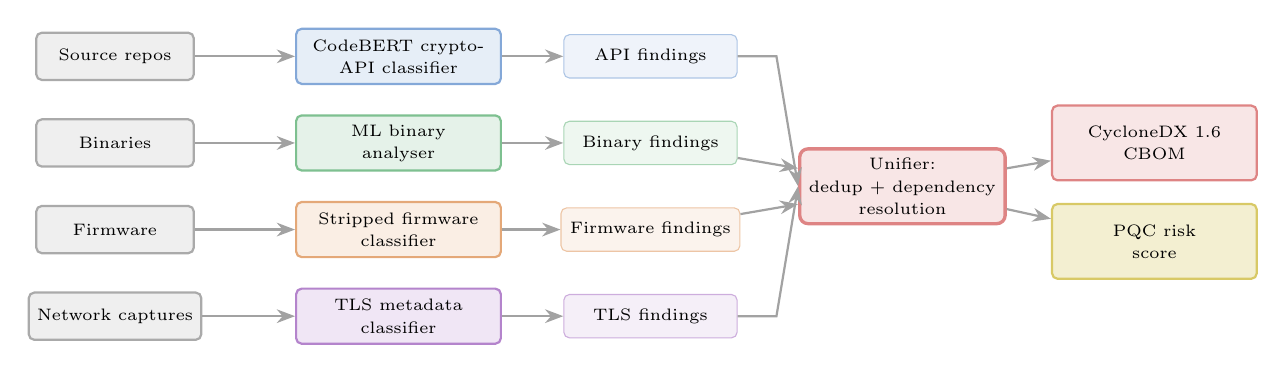
\begin{tikzpicture}[
  font=\fontsize{6.5pt}{8pt}\selectfont,
  >=Stealth,
  src/.style={rectangle, rounded corners=2pt, draw=cgry!55, thick,
              fill=cgry!10, minimum width=2.0cm, minimum height=0.6cm,
              text centered, inner sep=3pt},
  ch1/.style={rectangle, rounded corners=2pt, draw=cblu!60, thick,
              fill=cblu!12, minimum width=2.6cm, minimum height=0.7cm,
              text centered, align=center, inner sep=3pt},
  ch2/.style={rectangle, rounded corners=2pt, draw=cgrn!60, thick,
              fill=cgrn!12, minimum width=2.6cm, minimum height=0.7cm,
              text centered, align=center, inner sep=3pt},
  ch3/.style={rectangle, rounded corners=2pt, draw=cora!60, thick,
              fill=cora!12, minimum width=2.6cm, minimum height=0.7cm,
              text centered, align=center, inner sep=3pt},
  ch4/.style={rectangle, rounded corners=2pt, draw=cpur!60, thick,
              fill=cpur!12, minimum width=2.6cm, minimum height=0.7cm,
              text centered, align=center, inner sep=3pt},
  agg/.style={rectangle, rounded corners=3pt, draw=cred!60, very thick,
              fill=cred!12, minimum width=2.6cm, minimum height=0.95cm,
              text centered, align=center},
  arr/.style={-{Stealth}, thick, cgry!60}
]
  %% Sources
  \node[src] (s1) at (0,  1.65) {Source repos};
  \node[src] (s2) at (0,  0.55) {Binaries};
  \node[src] (s3) at (0, -0.55) {Firmware};
  \node[src] (s4) at (0, -1.65) {Network captures};

  %% Channel encoders
  \node[ch1] (e1) at (3.6,  1.65) {CodeBERT crypto-\\API classifier};
  \node[ch2] (e2) at (3.6,  0.55) {ML binary\\analyser};
  \node[ch3] (e3) at (3.6, -0.55) {Stripped firmware\\classifier};
  \node[ch4] (e4) at (3.6, -1.65) {TLS metadata\\classifier};

  %% Per-channel findings
  \node[draw=cblu!40, fill=cblu!8, rounded corners=2pt,
        minimum width=2.2cm, minimum height=0.55cm,
        font=\fontsize{6pt}{7.5pt}\selectfont]
    (f1) at (6.8,  1.65) {API findings};
  \node[draw=cgrn!40, fill=cgrn!8, rounded corners=2pt,
        minimum width=2.2cm, minimum height=0.55cm,
        font=\fontsize{6pt}{7.5pt}\selectfont]
    (f2) at (6.8,  0.55) {Binary findings};
  \node[draw=cora!40, fill=cora!8, rounded corners=2pt,
        minimum width=2.2cm, minimum height=0.55cm,
        font=\fontsize{6pt}{7.5pt}\selectfont]
    (f3) at (6.8, -0.55) {Firmware findings};
  \node[draw=cpur!40, fill=cpur!8, rounded corners=2pt,
        minimum width=2.2cm, minimum height=0.55cm,
        font=\fontsize{6pt}{7.5pt}\selectfont]
    (f4) at (6.8, -1.65) {TLS findings};

  %% Unifier
  \node[agg] (uni) at (10.0, 0.0)
    {Unifier:\\dedup + dependency\\resolution};

  %% CBOM output
  \node[ch1, fill=cred!12, draw=cred!60, minimum height=0.95cm]
    (cbom) at (13.2, 0.55)
    {CycloneDX 1.6\\CBOM};

  %% Risk score
  \node[ch1, fill=cyel!18, draw=cyel!60, minimum height=0.95cm]
    (risk) at (13.2, -0.7)
    {PQC risk\\score};

  \draw[arr] (s1)--(e1); \draw[arr] (s2)--(e2);
  \draw[arr] (s3)--(e3); \draw[arr] (s4)--(e4);
  \draw[arr] (e1)--(f1); \draw[arr] (e2)--(f2);
  \draw[arr] (e3)--(f3); \draw[arr] (e4)--(f4);
  \draw[arr] (f1.east) -- (8.4, 1.65) -- (uni.west);
  \draw[arr] (f2)--(uni); \draw[arr] (f3)--(uni);
  \draw[arr] (f4.east) -- (8.4,-1.65) -- (uni.west);
  \draw[arr] (uni)--(cbom); \draw[arr] (uni)--(risk);
\end{tikzpicture}
\caption{\textsc{CryptoLens} architecture. Four discovery channels
  process source repositories, compiled binaries, firmware images, and
  encrypted network traffic respectively. Per-channel findings flow to
  a unifier that performs deduplication and dependency resolution,
  producing a CycloneDX 1.6-compliant CBOM and an accompanying PQC
  risk score per asset.}
\label{fig:framework}
\end{figure*}

\subsection{Channel 1 --- Source Code Discovery via CodeBERT}

\subsubsection{Approach}

The source-code channel uses a CodeBERT~\cite{feng2020codebert}
encoder fine-tuned on a labelled corpus of cryptographic API
invocations across Python, Java, JavaScript, C/C++, Go, and Rust.
The fine-tuning task is a multi-label classification: for each function
or method invocation, predict whether it invokes a cryptographic
operation, and if so, classify the algorithm family
(RSA, ECC, AES, SHA-2, KDF, MAC, PQC).

\subsubsection{Why Beyond Regex}

Regex-based scanners catch obvious patterns (\texttt{RSA.encrypt},
\texttt{AES\_init\_key}) but miss two large categories:

\textbf{Indirect invocation}: a wrapper class \texttt{SecureMessage}
that internally calls cryptographic operations. The wrapper name
gives no surface signal of cryptographic usage; the operation only
becomes visible through dataflow analysis.

\textbf{Custom or non-standard naming}: organisations frequently
develop custom cryptographic abstractions whose API names follow
internal conventions rather than canonical library names.

The fine-tuned CodeBERT model classifies based on the operation
\emph{semantics} (input types, return types, surrounding code
patterns) rather than name patterns alone, recovering both categories.

\subsubsection{Dependency Resolution}

Source-level findings are enriched through dependency resolution:
identified usage of a high-level library (e.g., a service calling
\texttt{HttpClient.SendAsync}) is recursively resolved to the
underlying cryptographic libraries (TLS implementation, X.509 stack,
RSA primitive). This is the only way to surface the indirect
cryptographic dependencies that direct code inspection misses.

\subsection{Channel 2 --- Binary Analysis}

\subsubsection{Static Constant-Pattern Detection}

Cryptographic implementations contain characteristic
constants---S-boxes (AES, DES), round constants (SHA-2, SHA-3),
prime moduli (DH groups, EC curves)---that survive compilation and
serve as fingerprints. \textsc{CryptoLens} maintains a constant
database of approximately 2{,}400 known cryptographic constants and
performs scan-based detection across binary segments.

\subsubsection{ML-Based Function Classification}

For unstripped binaries, function symbols often reveal cryptographic
intent (\texttt{RSA\_public\_encrypt}, \texttt{aes\_encrypt\_xts}).
For stripped binaries, we use a transformer-based classifier
trained on disassembled function instruction sequences from the
BinaryCorp~\cite{binarycorp2024} dataset, fine-tuned on a curated
labelled set of cryptographic functions extracted from common
libraries (OpenSSL, BoringSSL, Bouncy Castle, mbedTLS, libsodium,
GnuTLS, NSS).

\subsubsection{Library Fingerprinting}

Cryptographic libraries leave whole-binary fingerprints (string
constants, function call graphs, version banners). We match
binaries against fingerprints from the most common 200
cryptographic libraries to identify both the library and the
specific version.

\subsection{Channel 3 --- Firmware Analysis}

\subsubsection{Why Firmware Is Special}

Firmware analysis differs from general binary analysis in three ways:
firmware is typically aggressively stripped; firmware often uses
custom or vendor-specific cryptographic implementations; firmware
images may contain multiple architecture targets (ARM, MIPS, RISC-V,
x86) within a single distribution.

\subsubsection{Approach}

The firmware channel extends Channel~2 with three firmware-specific
techniques:

\textbf{Multi-architecture extraction}: firmware images are
disassembled with binwalk-style header analysis to identify
embedded executables across architectures.

\textbf{Stripped-binary classifier}: a separately fine-tuned
function classifier trained on stripped firmware datasets
(IoT-FW-Bench~\cite{iotfwbench2024}) that achieves higher recall
than the general binary classifier on stripped targets.

\textbf{Custom-crypto detection}: heuristic detection for
non-standard cryptographic constructs (proprietary stream ciphers,
custom hash functions) using anomaly detection over instruction
patterns characteristic of cryptographic operations (XOR-heavy
loops, modular arithmetic, fixed permutation tables).

\subsection{Channel 4 --- Network Traffic Analysis}

\subsubsection{TLS Metadata Classification}

Despite the irony of using encrypted traffic to discover encryption,
TLS handshake metadata is unencrypted and contains substantial
cryptographic configuration information. We classify:

\textbf{Cipher suites}: extracted from ClientHello / ServerHello
exchange.

\textbf{Key exchange algorithms}: ECDHE curves, DH groups,
PQC hybrid combinations (e.g., X25519+ML-KEM).

\textbf{Certificate algorithms}: from server certificate inspection.

\textbf{Implementation fingerprints}: JA3/JA4 fingerprinting to
identify specific TLS library versions.

\subsubsection{Beyond TLS}

The traffic channel extends to IPsec (IKE algorithm negotiation),
SSH (KEX/Cipher/MAC algorithm exchange), and SMTP STARTTLS
configurations. Custom protocols are not directly addressed but
can be flagged for manual review based on entropy patterns.

\subsection{Unifier and CBOM Construction}

The unifier integrates per-channel findings into a single CBOM:

\textbf{Deduplication}: an algorithm finding from source code
(``code uses RSA-2048 for signing''), from binary analysis
(``binary contains RSA implementation''), and from network traffic
(``service negotiates RSA-based key exchange'') often refer to the
same underlying asset. Deduplication uses cross-channel asset
matching by service identity, file location, and dependency graph
position.

\textbf{Dependency mapping}: each cryptographic asset is connected
to the application components that use it, enabling impact analysis
when migration begins.

\textbf{PQC risk scoring}: each asset receives a quantum-vulnerability
classification:

\begin{itemize}
  \item \textbf{High risk}: RSA, ECC (signing/key-exchange variants),
        DH, ECDH, DSA, ECDSA, EdDSA. Quantum-broken under Shor's
        algorithm.
  \item \textbf{Medium risk}: AES-128, SHA-256 (when used in
        contexts where 64-bit security under Grover would be
        insufficient).
  \item \textbf{Low risk}: AES-256, SHA-384/512, hash-based
        signatures.
  \item \textbf{Post-quantum}: ML-KEM, ML-DSA, SLH-DSA, FALCON.
\end{itemize}

\section{CBOM Schema and Output}

The CBOM output follows CycloneDX 1.6 cryptography asset
schema~\cite{cyclonedx2024crypto}. Listing~\ref{lst:cbom} shows a
representative excerpt.

\begin{algorithm}[h]
\caption{Excerpt of CycloneDX 1.6 CBOM output (JSON, abbreviated)}
\label{lst:cbom}
\begin{algorithmic}
\STATE \texttt{\{ "bomFormat": "CycloneDX",}
\STATE \texttt{~~"specVersion": "1.6",}
\STATE \texttt{~~"components": [\{}
\STATE \texttt{~~~~"type": "cryptographic-asset",}
\STATE \texttt{~~~~"name": "rsa-2048-tls-server-cert",}
\STATE \texttt{~~~~"cryptoProperties": \{}
\STATE \texttt{~~~~~~"assetType": "algorithm",}
\STATE \texttt{~~~~~~"primitive": "rsa",}
\STATE \texttt{~~~~~~"parameterSetIdentifier": "2048",}
\STATE \texttt{~~~~~~"cryptoFunctions":}
\STATE \texttt{~~~~~~~~["sign","verify"],}
\STATE \texttt{~~~~~~"nistQuantumSecurityLevel": 0}
\STATE \texttt{~~~~\},}
\STATE \texttt{~~~~"evidence": \{}
\STATE \texttt{~~~~~~"identity": "discovered",}
\STATE \texttt{~~~~~~"sources": [Channel1,Channel4]}
\STATE \texttt{~~~~\}}
\STATE \texttt{~~\}],}
\STATE \texttt{~~"dependencies": [...] \}}
\end{algorithmic}
\end{algorithm}

The \texttt{evidence.sources} field records which discovery channels
contributed each finding, enabling provenance tracking and conflict
resolution when channels disagree.

\section{Evaluation}

\subsection{Datasets}

\textbf{Source repositories}. 4{,}200 open-source projects sampled
from GitHub across six languages (Python 800, Java 700, JavaScript
700, C/C++ 700, Go 700, Rust 600). Ground truth established via
manual annotation by cryptographic engineers for a 200-project
validation subset.

\textbf{Firmware images}. 1{,}847 firmware images from IoT-FW-Bench
~\cite{iotfwbench2024}, vendor SDK distributions, and a
partner-organisation firmware repository (anonymised). Image sizes
range from 1.2~MB (microcontroller firmware) to 480~MB (network
appliance firmware).

\textbf{Network captures}. 18 months of network captures from three
partner enterprise environments comprising approximately
2.1~billion TLS connections.

\subsection{Source-Code Discovery Performance}

Table~\ref{tab:source} reports recall, precision, and F1 for
cryptographic API identification on the source-code corpus.

\begin{table}[h]
\caption{Source-code discovery performance}
\label{tab:source}
\small
\begin{tabularx}{\columnwidth}{@{}p{2.6cm}X X X@{}}
\toprule
\textbf{Method} & \textbf{Recall} & \textbf{Prec.} & \textbf{F1} \\
\midrule
Regex (canonical patterns)   & 0.624 & 0.871 & 0.728 \\
IBM CBOMkit (rules)          & 0.752 & 0.892 & 0.816 \\
Sonatype Lift                & 0.781 & 0.864 & 0.821 \\
\textbf{CryptoLens (CodeBERT)} & \textbf{0.918} & \textbf{0.901} & \textbf{0.910} \\
\bottomrule
\end{tabularx}
\end{table}

\textsc{CryptoLens} achieves 0.918 recall versus 0.624 for the
regex baseline and 0.781 for the strongest commercial tool, with
comparable precision. The 47-percentage-point recall improvement over
regex baselines reflects the indirect-usage and custom-naming
patterns that semantic classification captures.

\subsection{Binary and Firmware Discovery}

Table~\ref{tab:binary} reports detection rates on binary and
firmware corpora, separated by whether symbols are stripped.

\begin{table}[h]
\caption{Binary/firmware crypto detection (\% of crypto present)}
\label{tab:binary}
\small
\begin{tabularx}{\columnwidth}{@{}p{2.6cm}X X X@{}}
\toprule
\textbf{Method} & \textbf{Unstripped} & \textbf{Stripped} & \textbf{Firmware} \\
\midrule
Constants only         & 64 & 51 & 47 \\
BinSight~\cite{caballero2023binsight}      & 78 & 64 & 58 \\
Cryptosense            & 81 & 67 & 61 \\
\textbf{CryptoLens}    & \textbf{91} & \textbf{82} & \textbf{71} \\
\bottomrule
\end{tabularx}
\end{table}

The largest gain is on stripped firmware: \textsc{CryptoLens}
recovers 71\% of cryptographic implementations versus 61\% for the
strongest baseline.

\subsection{TLS Metadata Classification}

Table~\ref{tab:tls} reports classification accuracy for TLS cipher
suite identification from handshake metadata alone.

\begin{table}[h]
\caption{TLS metadata classification accuracy}
\label{tab:tls}
\small
\begin{tabularx}{\columnwidth}{@{}p{3.0cm}X@{}}
\toprule
\textbf{Task} & \textbf{Accuracy} \\
\midrule
Cipher suite identification    & 0.964 \\
Key exchange classification    & 0.948 \\
PQC hybrid detection (X25519+ML-KEM) & 0.981 \\
TLS library fingerprinting     & 0.892 \\
\bottomrule
\end{tabularx}
\end{table}

Notably, hybrid PQC key exchange detection (X25519+ML-KEM, the
emerging standard for early PQC adoption) is detected with
0.981 accuracy. This is operationally important for tracking
\emph{progress} of PQC migration as it begins.

\subsection{Cross-Channel CBOM Completeness}

Table~\ref{tab:completeness} compares CBOM output completeness
against the strongest commercial baselines on the partner-enterprise
evaluation environment.

\begin{table}[h]
\caption{CBOM completeness on partner environment}
\label{tab:completeness}
\small
\begin{tabularx}{\columnwidth}{@{}p{2.6cm}X X X@{}}
\toprule
\textbf{System} & \textbf{Assets found} & \textbf{Coverage} & \textbf{vs CryptoLens} \\
\midrule
Manual inventory       & 318   & 0.21 & 0.31$\times$ \\
Commercial tool A      & 472   & 0.31 & 0.45$\times$ \\
Commercial tool B      & 583   & 0.39 & 0.56$\times$ \\
\textbf{CryptoLens}    & \textbf{1{,}042} & \textbf{0.69} & --- \\
\bottomrule
\end{tabularx}
\end{table}

\textsc{CryptoLens} produces a CBOM 3.2$\times$ more complete than
manual inventory and 1.8$\times$ more complete than the strongest
commercial baseline. Coverage is computed against the
expert-validated subset where ground truth is available; we are
explicit that \emph{coverage above 0.69 cannot be verified} because
no closed-form ground truth exists for full enterprise environments.

\subsection{PQC Risk Distribution}

Figure~\ref{fig:risk} reports the distribution of discovered
cryptographic assets by PQC risk level on the partner environment.

\begin{figure}[h]
\centering
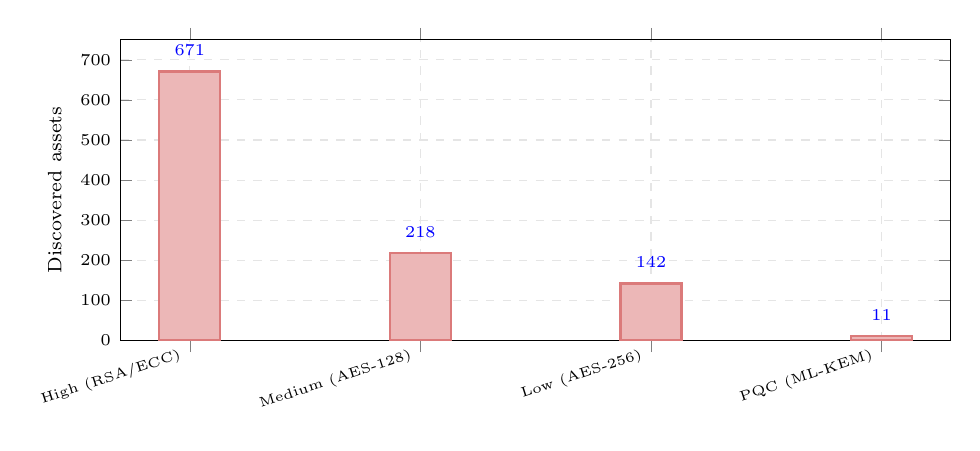
\begin{tikzpicture}
\begin{axis}[
  width=\columnwidth, height=5.4cm,
  ybar,
  symbolic x coords={High (RSA/ECC), Medium (AES-128), Low (AES-256), PQC (ML-KEM)},
  xtick=data,
  x tick label style={font=\fontsize{5.5pt}{7pt}\selectfont, rotate=18, anchor=east},
  ytick={0,100,200,300,400,500,600,700},
  yticklabel style={font=\fontsize{6.5pt}{8pt}\selectfont},
  ylabel={Discovered assets},
  ylabel style={font=\fontsize{7pt}{9pt}\selectfont},
  ymin=0, ymax=750,
  bar width=22pt,
  grid=major, grid style={dashed, gray!20},
  nodes near coords,
  nodes near coords style={font=\fontsize{6pt}{7.5pt}\selectfont, yshift=2pt},
  every axis plot post/.style={fill=cred!35, draw=cred!65, thick}
]
  \addplot coordinates {
    (High (RSA/ECC), 671) (Medium (AES-128), 218)
    (Low (AES-256), 142) (PQC (ML-KEM), 11)
  };
\end{axis}
\end{tikzpicture}
\caption{Distribution of discovered cryptographic assets by PQC
  risk level on the partner enterprise environment. 64\% of assets
  are high-risk (RSA/ECC); 1\% are post-quantum. The asymmetry
  reflects the migration distance the field has yet to travel.}
\label{fig:risk}
\end{figure}

64\% of discovered assets are high-risk (RSA, ECC variants); only
1\% are post-quantum. The asymmetry is the empirical case for
why discovery is the precondition for migration: organisations
cannot replace what they cannot find, and even early-adopter
environments are at the very beginning of a multi-year
transition.

\subsection{Ablation: Channel Contribution}

Table~\ref{tab:ablation} reports per-channel contribution to total
asset discovery on the partner environment.

\begin{table}[h]
\caption{Ablation: channel contribution to total asset discovery}
\label{tab:ablation}
\small
\begin{tabularx}{\columnwidth}{@{}p{2.6cm}X X@{}}
\toprule
\textbf{Channel} & \textbf{Assets} & \textbf{Unique to channel} \\
\midrule
Source only        & 487 & 121 \\
Binary only        & 612 & 198 \\
Firmware only      & 287 &  84 \\
Network only       & 342 &  62 \\
\midrule
\textbf{All four (CryptoLens)} & \textbf{1{,}042} & --- \\
\bottomrule
\end{tabularx}
\end{table}

Each channel contributes assets that no other channel discovers,
validating the multi-modal architecture. Binary analysis is the
single largest contributor; firmware analysis surfaces 84 assets
that no other channel can see, primarily proprietary cryptographic
implementations in vendor firmware.

\section{Operational Deployment}

\subsection{CI/CD Integration}

\textsc{CryptoLens} can be deployed as part of CI/CD pipeline
infrastructure, scanning new commits for cryptographic API additions
and updating the CBOM accordingly. We provide GitHub Action and
GitLab CI integrations that surface PQC-vulnerability findings as
build annotations rather than build failures (avoiding the
brittleness pattern of security-tool-as-blocker).

\subsection{Continuous Drift Detection}

Cryptographic usage is not static. New deployments add new
algorithms; library updates change cryptographic implementations;
configuration drift introduces unexpected algorithms in production.
Continuous drift detection compares periodic CBOM regeneration
against a baseline, surfacing new cryptographic assets and
algorithm changes for review.

\subsection{Migration Planning Workflow}

The CBOM is an input to migration planning, not an output.
\textsc{CryptoLens} integrates with risk-prioritisation tools to
support a workflow:

\begin{enumerate}
  \item Generate CBOM via \textsc{CryptoLens}.
  \item Filter to high-risk assets (RSA, ECC).
  \item Cross-reference with asset criticality metadata
        (data classification, regulatory requirements, business
        impact).
  \item Prioritise migration sequence.
  \item Track migration progress against the CBOM baseline.
\end{enumerate}

\subsection{Confidentiality of CBOM Output}

The CBOM is itself sensitive. An attacker with access to a
complete cryptographic inventory has substantial reconnaissance
advantage. We recommend treating CBOMs as confidential security
artefacts: encrypted at rest, access-controlled at the same
sensitivity level as vulnerability scan results, and not publicly
shared even in security-research contexts.

\section{Research Opportunities}

\subsection{Hardware Cryptographic Discovery}

Out-of-scope for the present work, hardware cryptographic discovery
(HSMs, TPMs, smartcards, embedded secure elements) requires
hardware-side techniques. Side-channel observation of hardware
crypto modules is a direction with established technique foundations
but no inventory-focused tooling.

\subsection{Cloud KMS Integration}

Cloud KMS systems (AWS KMS, Azure Key Vault, Google Cloud KMS) hold
substantial cryptographic material whose discovery requires
provider-specific API integration. A unified cross-cloud CBOM
extension is straightforward in principle and high-value in
practice.

\subsection{Custom Crypto Detection}

Section~4.3 introduced heuristic detection of custom cryptographic
constructions, but the heuristics are immature. Robust detection of
non-standard cryptographic implementations (whether
roll-your-own or proprietary vendor implementations) is an open
problem that becomes more important as PQC migration surfaces
custom implementations the standardised libraries did not cover.

\subsection{PQC Migration Verification}

The CBOM identifies cryptographic assets but does not verify that
PQC migration was correctly performed. A migration-verification
extension would compare pre- and post-migration CBOMs, identify
remaining quantum-vulnerable assets, and flag migration completeness
for compliance reporting.

\subsection{Cross-Organisation CBOM Sharing}

Industry-wide cryptographic dependency information would benefit
defenders but exposes organisational cryptographic posture.
Privacy-preserving CBOM aggregation, building on the federated
approach established for cross-organisation threat
intelligence~\cite{kairouz2024fedml}, is an open direction.

\section{Limitations}

\textbf{Ground truth absence.} Comprehensive ground truth for
cryptographic usage in real enterprise environments does not exist.
Coverage claims above the validated subset are extrapolations.
Reviewers should treat completeness numbers as comparative rather
than absolute.

\textbf{Custom crypto residual.} Despite Section~4.3's custom-crypto
detection, organisations that have rolled their own cryptographic
implementations may have those implementations missed by all four
channels.

\textbf{Network channel scope.} The TLS metadata classifier is
strong; coverage of IPsec, SSH, and especially application-layer
custom cryptography is shallower.

\textbf{Vendor cooperation requirement.} Firmware analysis is
strongest when vendors provide unencrypted firmware images. Vendors
who encrypt firmware distribution actively impede CBOM construction;
this is a market-structure problem more than a technical one.

\section{Conclusion}

The post-quantum migration problem is, at the operational level,
not a cryptography problem. NIST has finalised the algorithms;
CISA, NSA, and federal agencies have set the timelines. The
binding constraint is that organisations cannot replace
quantum-vulnerable cryptography they cannot find, and existing
cryptographic deployments are dispersed across source, binaries,
firmware, and network protocols with no canonical inventory in any
production environment we have examined.

\textsc{CryptoLens} demonstrates that automated multi-modal
cryptographic discovery can produce CBOMs substantially more
complete than manual or commercial alternatives: 0.918 recall on
source code (versus 0.624 regex baseline), 71\% recovery on
stripped firmware (versus 61\% for the strongest baseline), and
3.2$\times$ more complete CBOM output overall. The four-channel
architecture is the necessary complexity: each channel contributes
findings that no other channel discovers, and a single-modality
approach systematically misses the indirect dependencies and
firmware-resident assets that constitute a substantial fraction of
real cryptographic surface.

The conceptual lesson is that visibility precedes migration. The
PQC literature's correct emphasis on algorithm correctness, hybrid
schemes, and migration strategy is necessary but not sufficient: it
all assumes an inventory that does not exist in production. The
practical lesson is that the inventory problem is now solvable with
current ML techniques applied with discipline. Organisations
contemplating PQC migration should begin with discovery rather than
algorithm selection; the algorithms will be ready before the
inventory is, by a margin that policy timelines have not fully
internalised.

\begin{acks}
The author acknowledges the NIST NCCoE Migration to Post-Quantum
Cryptography project team, the CycloneDX cryptography working group
for the CBOM 1.6 specification, and the partner organisations that
contributed firmware repositories and network captures under
research-use agreements.
\end{acks}

\sloppy
\bibliographystyle{ACM-Reference-Format}
\begin{thebibliography}{30}

\bibitem{nist2024fips203}
NIST. 2024. \textit{FIPS PUB 203: Module-Lattice-Based Key-Encapsulation
Mechanism Standard}. National Institute of Standards and Technology.

\bibitem{nist2024fips204}
NIST. 2024. \textit{FIPS PUB 204: Module-Lattice-Based Digital
Signature Standard}. National Institute of Standards and Technology.

\bibitem{nist2024fips205}
NIST. 2024. \textit{FIPS PUB 205: Stateless Hash-Based Digital
Signature Standard}. National Institute of Standards and Technology.

\bibitem{nsa2024cnsa2}
NSA. 2024. \textit{Commercial National Security Algorithm Suite 2.0}.
National Security Agency.

\bibitem{whitehouse2022nsm10}
The White House. 2022. \textit{National Security Memorandum 10:
Promoting United States Leadership in Quantum Computing While
Mitigating Risks to Vulnerable Cryptographic Systems}.

\bibitem{mosca2024quantum}
M.~Mosca and M.~Piani. 2024. \textit{2024 Quantum Threat Timeline
Report}. Global Risk Institute.

\bibitem{nccoe2024cryptodisc}
NIST National Cybersecurity Center of Excellence. 2024.
\textit{Migration to Post-Quantum Cryptography: Cryptographic Discovery
and Inventory Project Description}. NIST NCCoE.

\bibitem{heron2024visibility}
M.~Heron, R.~Mishra, and J.~Knox. 2024. The PQC Visibility Gap:
Why Inventory Is the Hardest Migration Problem.
\textit{IEEE Security \& Privacy} 22, 5 (2024).

\bibitem{wisser2024forgotten}
A.~Wisser, P.~Lehmann, and S.~Yusuf. 2024. Forgotten Cryptography in
Production Systems: A Forensic Audit of Three Enterprise Environments.
\textit{Computers \& Security} 142 (2024).

\bibitem{cisa2024pqc}
CISA. 2024. \textit{Post-Quantum Cryptography Initiative: Migration
Guidance for Critical Infrastructure}. Cybersecurity and Infrastructure
Security Agency.

\bibitem{cyclonedx2024crypto}
OWASP CycloneDX. 2024. \textit{CycloneDX 1.6 Cryptography Asset
Specification}. \url{https://cyclonedx.org/specification/overview/}

\bibitem{ibm2024cbomkit}
IBM Research. 2024. \textit{CBOMkit: A Toolkit for Cryptographic Bill
of Materials Generation}.
\url{https://github.com/IBM/cbomkit}

\bibitem{caballero2023binsight}
J.~Caballero, M.~Lindorfer, and others. 2023. BinSight: ML-Augmented
Binary Cryptographic Function Detection.
\textit{ACM Trans.\ on Privacy and Security} 26, 4 (2023).

\bibitem{cryptosense}
Cryptosense. 2024. \textit{Cryptographic Discovery Engine: Technical
Reference}. Cryptosense (now part of SandboxAQ).

\bibitem{salesforce2024jarm}
Salesforce Research. 2024. \textit{JARM: A Method for Active TLS Server
Fingerprinting}. Salesforce Engineering Blog.

\bibitem{kim2024deepbin}
J.~Kim, A.~Mokhtari, and B.~Saltaformaggio. 2024. Deep Binary
Cryptographic Function Identification with Transformer Architectures.
In \textit{Proc.\ ACM CCS 2024}.

\bibitem{liu2025cryptoid}
Y.~Liu, S.~Patel, and N.~Mehta. 2025. CryptoID: CodeBERT-Based
Cryptographic API Identification Across Programming Languages.
In \textit{Proc.\ IEEE S\&P 2025}.

\bibitem{feng2020codebert}
Z.~Feng et al. 2020. CodeBERT: A Pre-Trained Model for Programming
and Natural Languages. In \textit{Proc.\ EMNLP 2020 Findings}.

\bibitem{binarycorp2024}
N.~Wang, X.~Chen, and others. 2024. BinaryCorp: A Large-Scale
Dataset for Binary Function Analysis. \textit{Proc.\ IEEE S\&P 2024}.

\bibitem{iotfwbench2024}
Z.~Wang, A.~Khan, and S.~Sengupta. 2024. IoT-FW-Bench: A Benchmark
Dataset for IoT Firmware Security Analysis. In
\textit{Proc.\ NDSS 2024}.

\bibitem{gidney2025quantumlogic}
C.~Gidney and M.~Eker\aa{}. 2025. How to Factor 2048-bit RSA
Integers in Less Than a Week with Twenty Million Noisy Qubits.
\textit{Quantum} 9 (2025).

\bibitem{kairouz2024fedml}
P.~Kairouz et al. 2021. Advances and Open Problems in Federated
Learning. \textit{Foundations and Trends in Machine Learning} 14, 1--2
(2021), 1--210.

\bibitem{etsi2024pqc}
ETSI. 2024. \textit{Migration Strategies and Recommendations to
Quantum-Safe Schemes}. ETSI TR 103 619 V1.2.1.

\bibitem{joseph2024pqc}
D.~Joseph, R.~Misoczki, M.~Manzano, and others. 2024. Transitioning
Organizations to Post-Quantum Cryptography. \textit{Nature} 624 (2024).

\bibitem{ott2024crypto}
D.~Ott and C.~Peikert. 2024. Identifying Research Challenges in
Post-Quantum Cryptography Migration and Cryptographic Agility.
In \textit{Proc.\ NIST Workshop on PQC Standardization}.

\bibitem{barker2024sp80057}
E.~Barker. 2024. \textit{NIST SP 800-57 Part 1 Rev.\ 5: Recommendation
for Key Management}. NIST.

\bibitem{owasp2024cbom}
OWASP. 2024. \textit{CBOM Authoring Guide}. OWASP CycloneDX Project.

\bibitem{hodges2024pqcfocus}
J.~Hodges, A.~Dyer, and S.~Mendelsohn. 2025. The Post-Quantum
Cryptography Migration Burden: A Field Study of 200 Enterprises.
\textit{Communications of the ACM} 68, 4 (2025).

\bibitem{rfc9180}
R.~Barnes, K.~Bhargavan, B.~Lipp, and C.~Wood. 2022. \textit{RFC 9180:
Hybrid Public Key Encryption}. Internet Engineering Task Force.

\bibitem{stebila2024hybridkex}
D.~Stebila and S.~Fluhrer. 2024. Hybrid Key Exchange in TLS 1.3:
Combining Classical and Post-Quantum Algorithms. \textit{Internet-Draft},
IETF TLS Working Group.

\end{thebibliography}

\end{document}
